% Drawing 138/06-47 -- folder 138, batch 06, archive page 118 (PDF page 119).
% Transcription: à gauche, petites cartes d'une autre encre : $(\alpha)$ une boucle traversée d'un segment, $\mathbb{Z}_2$ ; $(\gamma)$ une petite croix dans un cercle, $\mathbb{Z}_2$ ; $(\beta)$ deux boucles accolées, $\mathbb{Z}_2$. Puis : un segment à deux sommets suivi d'une fourche, $\mathbb{Z}_2$ ; un segment suivi d'une boucle avec arête, $1$ ; un segment suivi d'une boucle, $\mathbb{Z}_2$.
% Kind: table of small maps with automorphism groups (degree 6, c). Method 2 (schematic redraw from the facsimile). Status: ok.
% Notes: At the left, small maps in another ink: (alpha) a loop crossed by a segment, Z_2; (gamma) a small cross in a circle, Z_2; (beta) two joined loops, Z_2. Then: a segment with two vertices followed by a fork, Z_2; a segment followed by a loop with an edge, 1 (circled); a segment followed by a loop, Z_2. Each small map carries its automorphism group as written (given as labels, since the transcription names them); vertex positions and loop shapes approximate.
% Coordinates: 1 unit = 1 mm = 1/100 of the crop width (bbox in page fractions: [0.097, 0.483, 0.886, 0.596]).
% Redrawn by Claude (claude-opus-5-5), issue #73, 2026-11-07; not checked by a human; not compiled (no TeX in the session).
% Rights: reproduces part of the work -- behind RENDER_TRANSCRIPTS, never published by itself.
\documentclass[tikz,border=3pt]{standalone}
\usepackage{amsmath,amssymb}
\usetikzlibrary{patterns,arrows.meta}
\tikzset{pencil/.style={black!45}, struck/.style={black!35}, mark/.style={circle,draw,inner sep=1.3pt}, pt/.style={circle,fill,inner sep=0.9pt}, opt/.style={circle,draw,fill=white,inner sep=1.1pt}}
\begin{document}
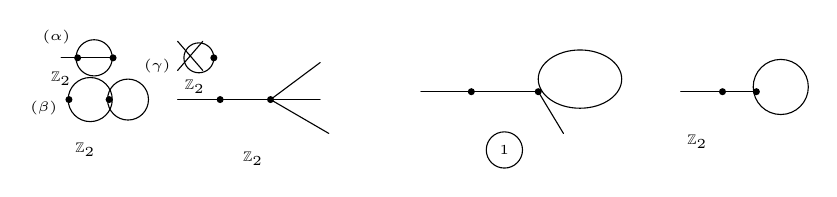
\begin{tikzpicture}[x=1mm,y=1mm,line cap=round,line join=round,font=\scriptsize]
\draw (8.5,-5.3) circle[radius=2.3];
\draw (4.3,-5.3) -- (10.9,-5.3);
\node[pt] at (6.4,-5.3) {};
\node[pt] at (10.9,-5.3) {};
\node[inner sep=1pt] at (3.7,-2.7) {\tiny $(\alpha)$};
\node[inner sep=1pt] at (4.3,-8) {\tiny $\mathbb{Z}_2$};
\draw (21.8,-5.3) circle[radius=1.9];
\draw (19.1,-3.2) -- (22.3,-6.9);
\draw (19.1,-6.9) -- (22.3,-3.2);
\node[pt] at (23.7,-5.3) {};
\node[inner sep=1pt] at (16.5,-6.4) {\tiny $(\gamma)$};
\node[inner sep=1pt] at (21.3,-9) {\tiny $\mathbb{Z}_2$};
\draw (8,-10.6) circle[radius=2.8];
\draw (12.8,-10.6) circle[radius=2.6];
\node[pt] at (5.3,-10.6) {};
\node[pt] at (10.4,-10.6) {};
\node[inner sep=1pt] at (2.1,-11.7) {\tiny $(\beta)$};
\node[inner sep=1pt] at (7.4,-17) {\tiny $\mathbb{Z}_2$};
\draw (19.1,-10.6) -- (30.9,-10.6);
\draw (30.9,-10.6) -- (37.2,-5.9);
\draw (30.9,-10.6) -- (38.3,-14.9);
\draw (30.9,-10.6) -- (37.2,-10.6);
\node[pt] at (24.5,-10.6) {};
\node[pt] at (30.9,-10.6) {};
\node[inner sep=1pt] at (28.7,-18.1) {\tiny $\mathbb{Z}_2$};
\draw (50,-9.6) -- (64.9,-9.6);
\draw (70.2,-8) ellipse[x radius=5.3, y radius=3.7];
\draw (64.9,-9.6) -- (68.1,-14.9);
\node[pt] at (56.4,-9.6) {};
\node[pt] at (64.9,-9.6) {};
\draw (60.6,-17) circle[radius=2.3];
\node[inner sep=1pt] at (60.6,-17) {\tiny $1$};
\draw (83,-9.6) -- (92.6,-9.6);
\draw (95.7,-9) circle[radius=3.5];
\node[pt] at (88.3,-9.6) {};
\node[pt] at (92.6,-9.6) {};
\node[inner sep=1pt] at (85.1,-16) {\tiny $\mathbb{Z}_2$};
\end{tikzpicture}
\end{document}
